\documentclass[12pt]{article}
\usepackage{amsmath,amssymb,bookmark,graphicx,parskip,custom}
\usepackage[margin=.8in]{geometry}
\allowdisplaybreaks
\hypersetup{colorlinks,
    citecolor=black,
    filecolor=black,
    linkcolor=black,
    urlcolor=black
}
\setcounter{secnumdepth}{5}

\begin{document}

\title{Git}
\author{Kevin Carruthers, Lara Janecka, Nik Klassen, Eric Pemberton}
\date{\vspace{-2ex}Fall 2015}
\maketitle\HRule

\tableofcontents
\newpage

\section{System Functionality}

\section{Quality Attributes and Scenarios}

\section{Architectural Views}
\subsection{File Structure}
\begin{figure}[htbp]
\centering
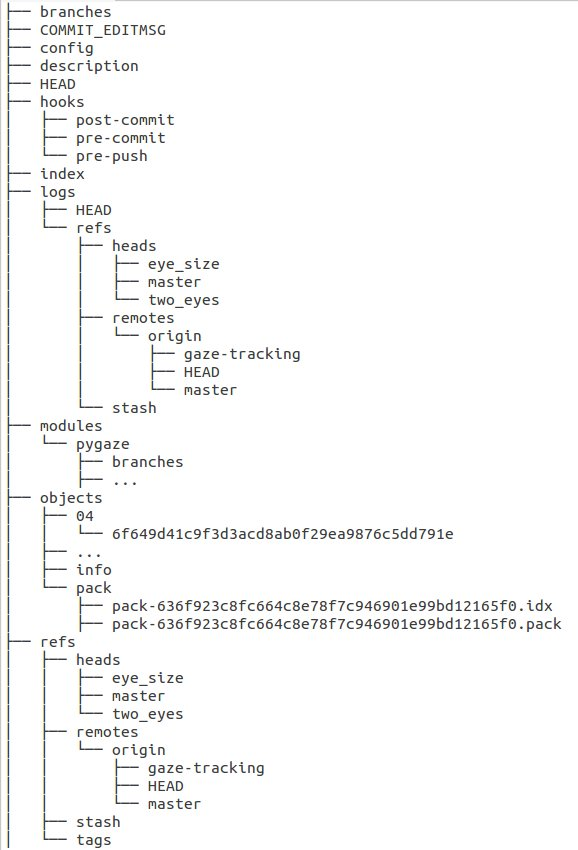
\includegraphics[width=0.5\textwidth]{filestructure.jpeg}
\caption{File structure of .git folder}
\label{fig:file}
\end{figure}

Figure~\ref{fig:file} displays the file structure of the .git folder for one group members SE390 internal miniproject. The git file structure is broken up into numerous sub folders used to manipulate the git tree.

\begin{description}
\item[The branches folder] contains information needed to manage branches (this is deprecated so the folder is empty).
\item[The COMMIT\_EDITMSG] file stores the last commit message.
\item[The config folder] contains the git configuration specific to this project. This example did not have any project specific configurations so the folder is empty.
\item[The description folder] is empty because it is used to contain information necessary for viewing the repository through a web client -- this was not used for this project.
\item[The HEAD file] stores a reference to which branch you are currently on, and
\item[The hooks folder] contains scripts to be executed on triggers defined by its subfolders post-commit, pre-commit, and pre-push.
\item[The index] contains information of what changes have been ``added'' and will be committed when the user runs the commit command.
\item[The logs folder] contains all changes that have been made in the history of the repository.
\item[The modules folder] outlines submodules that were included. In the example given it is seen as the pygaze module which contains the .git folder for that module so that git knows how to interact with it.
\item[The objects folder] stores all git objects (the hierarchy of these can be seen in Figure~\ref{fig:objects}) referenced by their SHA.
\item[The refs folder] contains references to all local heads (corresponding to all local branches) and all remote heads (corresponding to all remote branches).
\end{description}

Note that the index and logs folders do not contain the same data: the index only contains information that has been added and not committed.

The history of the git repository is stored by reference which are heads (referring to the heads of branches the names of which are the subfolders) or remotes (referring to branches that have been pushed).

\subsection{Object Structure}
\begin{figure}[htbp]
\centering
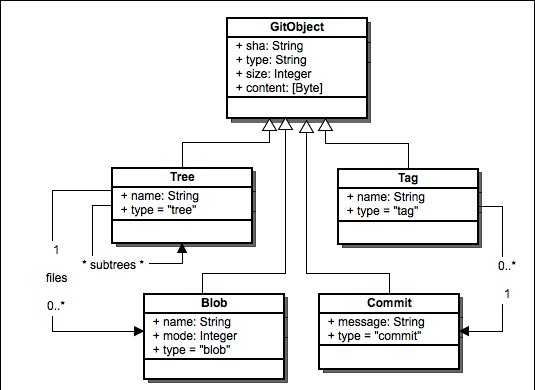
\includegraphics[width=0.95\textwidth]{objects.jpeg}
\caption{Object hierarchy for git}
\label{fig:objects}
\end{figure}

Git manages repositories through a tree of git objects. The UML for this is in Figure~\ref{fig:objects}. All objects are contain a large string called its sha through which you can reference that object. All content in a repository is stored in Blob objects and ordered into a tree objects. Each Blob represents a file stored in memory. The tree structure represents a directory. Commit objects point at the tree representing the top level directory of the commit. Tags are objects pointing to a single commit for use by the repository history.

\section{Architectural Analysis}

\section{Key Weaknesses}
Since git is written as a nested script-based architecture, it is not designed to be library-first; that is, the git implementation is designed to be executed as-is rather than imported into other tools. This can cause problems in the cases of, for example, IDEs, which thus can not simply import the specific submodule they desire but must instead execute the script as a forked process. This could be fixed by designing git as a library-first application and simply calling the various module entry-points from a shell script (in order to maintain the current interface).

Additionally, since the git modules are designed in the tree-based fashion outlined above, the architecture may be difficult for new users to comprehend. When they are searching for the method to perform some task, new users must try each submodule until they find the correct one. This could be addressed by merging similar submodules in order to try to make the system simpler, though this may have the side-effect of creating a system which is less powerful and customizable to more advanced users.

\section{References}
\begin{itemize}
\item https://www.siteground.com/tutorials/git/directory.htm
\item http://aosabook.org/en/git.html
\end{itemize}

\end{document}
